\documentclass[tikz,border=5pt]{standalone}
\begin{document}
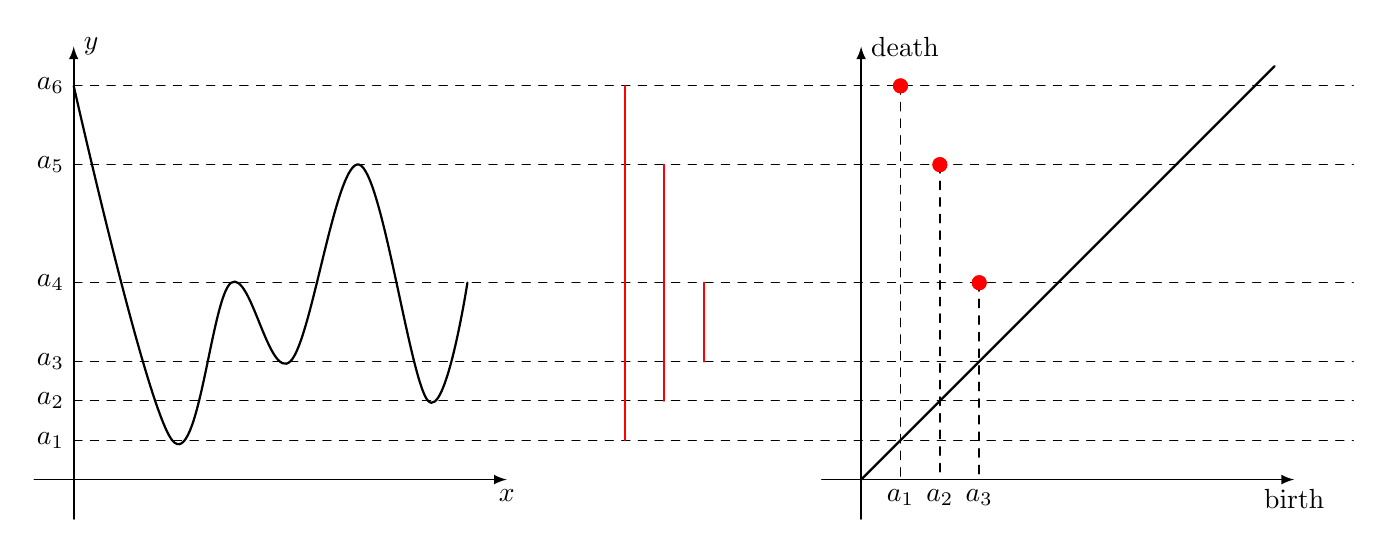
\begin{tikzpicture}[line cap=round,scale=5]
\def\a{.1}
\def\b{.2}
\def\c{.3}
\def\d{.5}
\def\e{.8}
\def\f{1}
\draw[thick] plot[smooth,tension=.6] coordinates {(0,\f) (.25,\a) (.4,\d) (.55,\c) (.725,\e) (.9,\b) (1,\d)};

\draw[-latex,semithick] (-.1,0) -- (1.1,0) node[below] {$x$};
\draw[-latex,semithick] (0,-.1) -- (0,1.1) node[right] {$y$};
\foreach \i[count = \j from 1] in {\a,\b,\c,\d,\e,\f} {
  \draw[dashed] (0,\i) node[left] {$a_\j$} -- ++(3.25,0) ;
}

\foreach \i/\j/\xpos in {\a/\f/1.4,\b/\e/1.5,\c/\d/1.6}{
    \draw[red,thick] (\xpos,\i) -- (\xpos,\j);
}

\begin{scope}[xshift=2cm]
\draw[-latex,semithick] (-.1,0) -- (1.1,0) node[below] {birth};
\draw[-latex,semithick] (0,-.1) -- (0,1.1) node[right] {death};
\draw[thick] (0,0) -- (1.05,1.05);
\draw[radius=.5pt,red,fill=red] (\a,\f) circle[] (\b,\e) circle[] (\c,\d) circle[];
\foreach \i/\j[count = \k from 1] in {\a/\f,\b/\e,\c/\d} {
    \draw[dashed,semithick] (\i,\j) -- (\i,0) node[below] {$a_\k$};
    \draw[red,fill=red] (\i,\j) circle[radius=.5pt];
}
\end{scope}
\end{tikzpicture}
\end{document}